Se realizo un Modelo de Entidad Relación y Modelo Relacional derivado, los cuales fueron utilizados para implementar la solución. \\

A continuación se muestra el MER realizado:\\

\vspace*{0.3cm} \vspace*{0.3cm}
  \begin{center}
 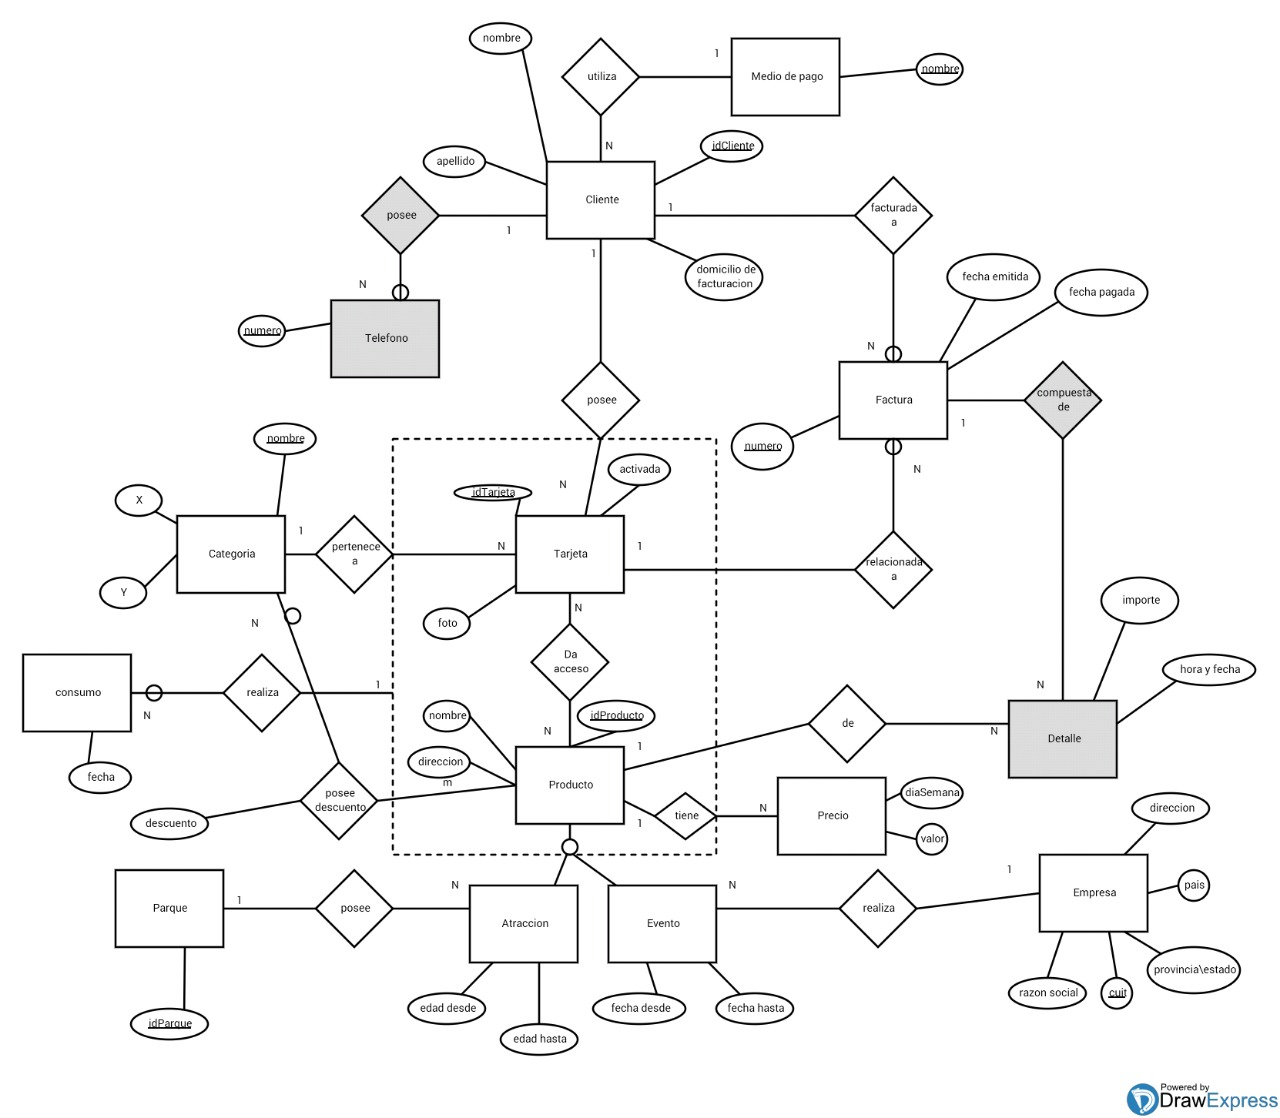
\includegraphics[scale=0.43]{der.jpeg}
 {$Gr$\'a$fico$ $Modelo$ $Entidad$ $Relaci$\'o$n$}
  \end{center}
  \vspace*{0.3cm}
  
En base al MER realizado se derivan las siguientes tablas con sus respectivos atributos y claves:\\

\textbf{Cliente}(\underline{idCliente}, nombre, apellido, domicilioFact)\\
PK =  $\lbrace$idCliente$\rbrace$  \\
\textbf{Telefono}(\underline{idCliente}, telefono)\\
PK = $\lbrace$idCliente, telefono$\rbrace$ FK = $\lbrace$idCliente$\rbrace$\\
\textbf{MedioDePago}(\underline{idCliente, idMedioDePago}, nombre)\\
PK = $\lbrace$idCliente, idMedioDePago$\rbrace$ FK = $\lbrace$idCliente$\rbrace$\\
\textbf{factura}(\underline{tipo, num, idCliente}, fechaEmitida, fechaVencimiento, medioDePago)\\
PK = $\lbrace$tipo, num, idCliente$\rbrace$ FK = $\lbrace$idCliente$\rbrace$\\
\textbf{detalle}(\underline{tipo, num, idDetalle}, importe, horaYFecha, detalle,)\\
PK = $\lbrace$tipo,num,idDetalle$\rbrace$ FK = $\lbrace$tipo,num$\rbrace$\\
\textbf{recibo}(\underline{tipo, num, idRecibo}, precioPagado)\\
PK = $\lbrace$tipo, num, idRecibo$\rbrace$ FK = $\lbrace$tipo,num$\rbrace$\\
\textbf{Empresa}(\underline{idEmpresa, idEvento}, cuit, razonSocial, pais, direccion, provincia/estado)\\
PK = $\lbrace$idEmpresa, idEvento$\rbrace$ FK = $\lbrace$idEvento$\rbrace$\\
